\begin{figure}[t]
  \center
  \def\layersep{3cm}
  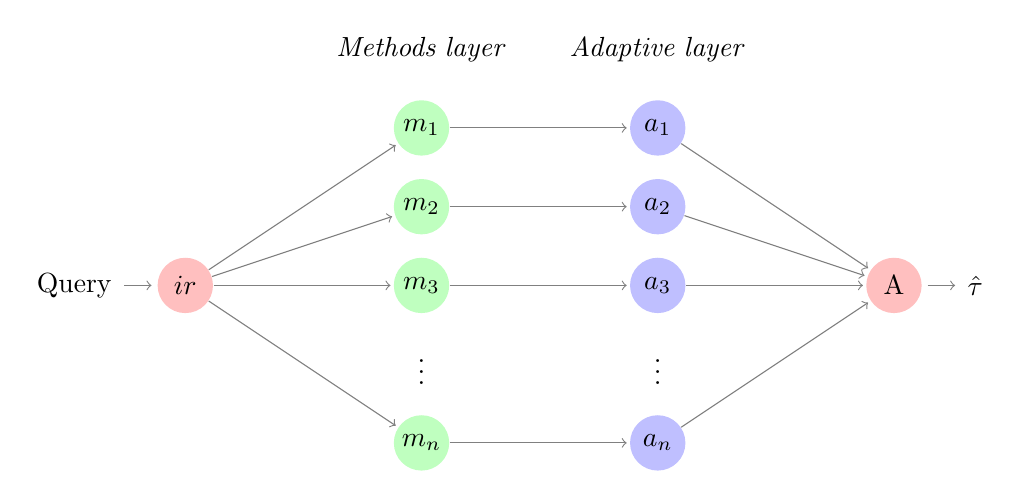
\begin{tikzpicture}[shorten >=1pt,->,draw=black!50, node distance=\layersep]

    \tikzstyle{every pin edge}=[<-,shorten <=2pt]
    \tikzstyle{neuron}=[circle,fill=black!25,minimum size=20pt,inner sep=0pt]
    \tikzstyle{input neuron}=[neuron, fill=green!25];
    \tikzstyle{output neuron}=[neuron, fill=red!25];
    \tikzstyle{hidden neuron}=[neuron, fill=blue!25];
    \tikzstyle{txt}=[neuron, fill=white];
    \tikzstyle{annot} = [text width=10em, text centered]
    
    \node[output neuron, pin=left:Query] (IR) at (0,-3) {$ir$};
    
    \node[input neuron] (M-1) at (\layersep, -1) {$m_1$};
    \node[input neuron] (M-2) at (\layersep, -2) {$m_2$};
    \node[input neuron] (M-3) at (\layersep, -3) {$m_3$};
    \node[txt] (M-N) at (\layersep, -4) {$\vdots$};
    \node[input neuron] (M-4) at (\layersep, -5) {$m_n$};
    
    \node[hidden neuron] (E-1) at (\layersep*2, -1) {$a_1$};
    \node[hidden neuron] (E-2) at (\layersep*2, -2) {$a_2$};
    \node[hidden neuron] (E-3) at (\layersep*2, -3) {$a_3$};
    \node[txt] (E-N) at (\layersep*2, -4) {$\vdots$};
    \node[hidden neuron] (E-4) at (\layersep*2, -5) {$a_n$};
    
    \node[output neuron,pin={[pin edge={->}]right:$\hat{\tau}$}, right of=E-3] (O) {A};
    
    \foreach \source in {1,...,4}
         \path (M-\source) edge (E-\source);
     
    \foreach \source in {1,...,4}
         \path (IR) edge (M-\source);
 
    \foreach \source in {1,...,4}
         \path (E-\source) edge (O);
    
    \node[annot, above of=M-1, node distance=1cm] (hl) {\emph{Methods layer}};
    \node[annot, right of=hl] {\emph{Adaptive layer}};

  \end{tikzpicture}

  \vspace{1em}
  \caption[Stacked Rank Aggregation]{
    Stacked Rank Aggregation: 
    An IR method returns a results list of possibly related items, each with a ranking score.
    The methods layer estimates ratings for each item in the results list.
    The adaptive layer predicts how accurate ach of these ratings are likely to be.
    Finally, the ranking scores, ratings and accuracy estimations are combined
    into one result list, $\hat{\tau}$.
  }
  \label{fig:adaptiverank}
\end{figure}
